\graphicspath{{images/}}
\chapter{2020-06-02}
%\textbf{Checklist}
%\begin{todolist}
 %   \item[\done] Create test triples to evaluate learned relation embeddings (evaluate on relation type prediction).
%    \item[\done] Visualization1: Use tensorboard to draw the training curves for loss $L_e$, $L_r$, and $L_p$ on both train and dev. (note: train curves are drawn, dev curves of $L_r$ still have some problem (need to figure out why.)) 
%    \item[\done] Loss modification: Add entropy constraint for relation distribution $\alpha$. We hope the $\alpha$ to be inclined to one label, so the entropy of $\alpha$ should be small. 
%   \item[\done] Try learning a weight for the loss components
%    \item Visualization2: use TSNE to visualize $\alpha$. 
%    \item May try different kinds of negative sampling strategy, eg., sample nodes with similar degeree or similar frequency. 
%    \item Hidden units for relation classifier needs to be tuned. Now the $h \in R^{100}$, $t \in R^{100}$, $W \in R^{100}$
%\end{todolist}

%\section{Summary}
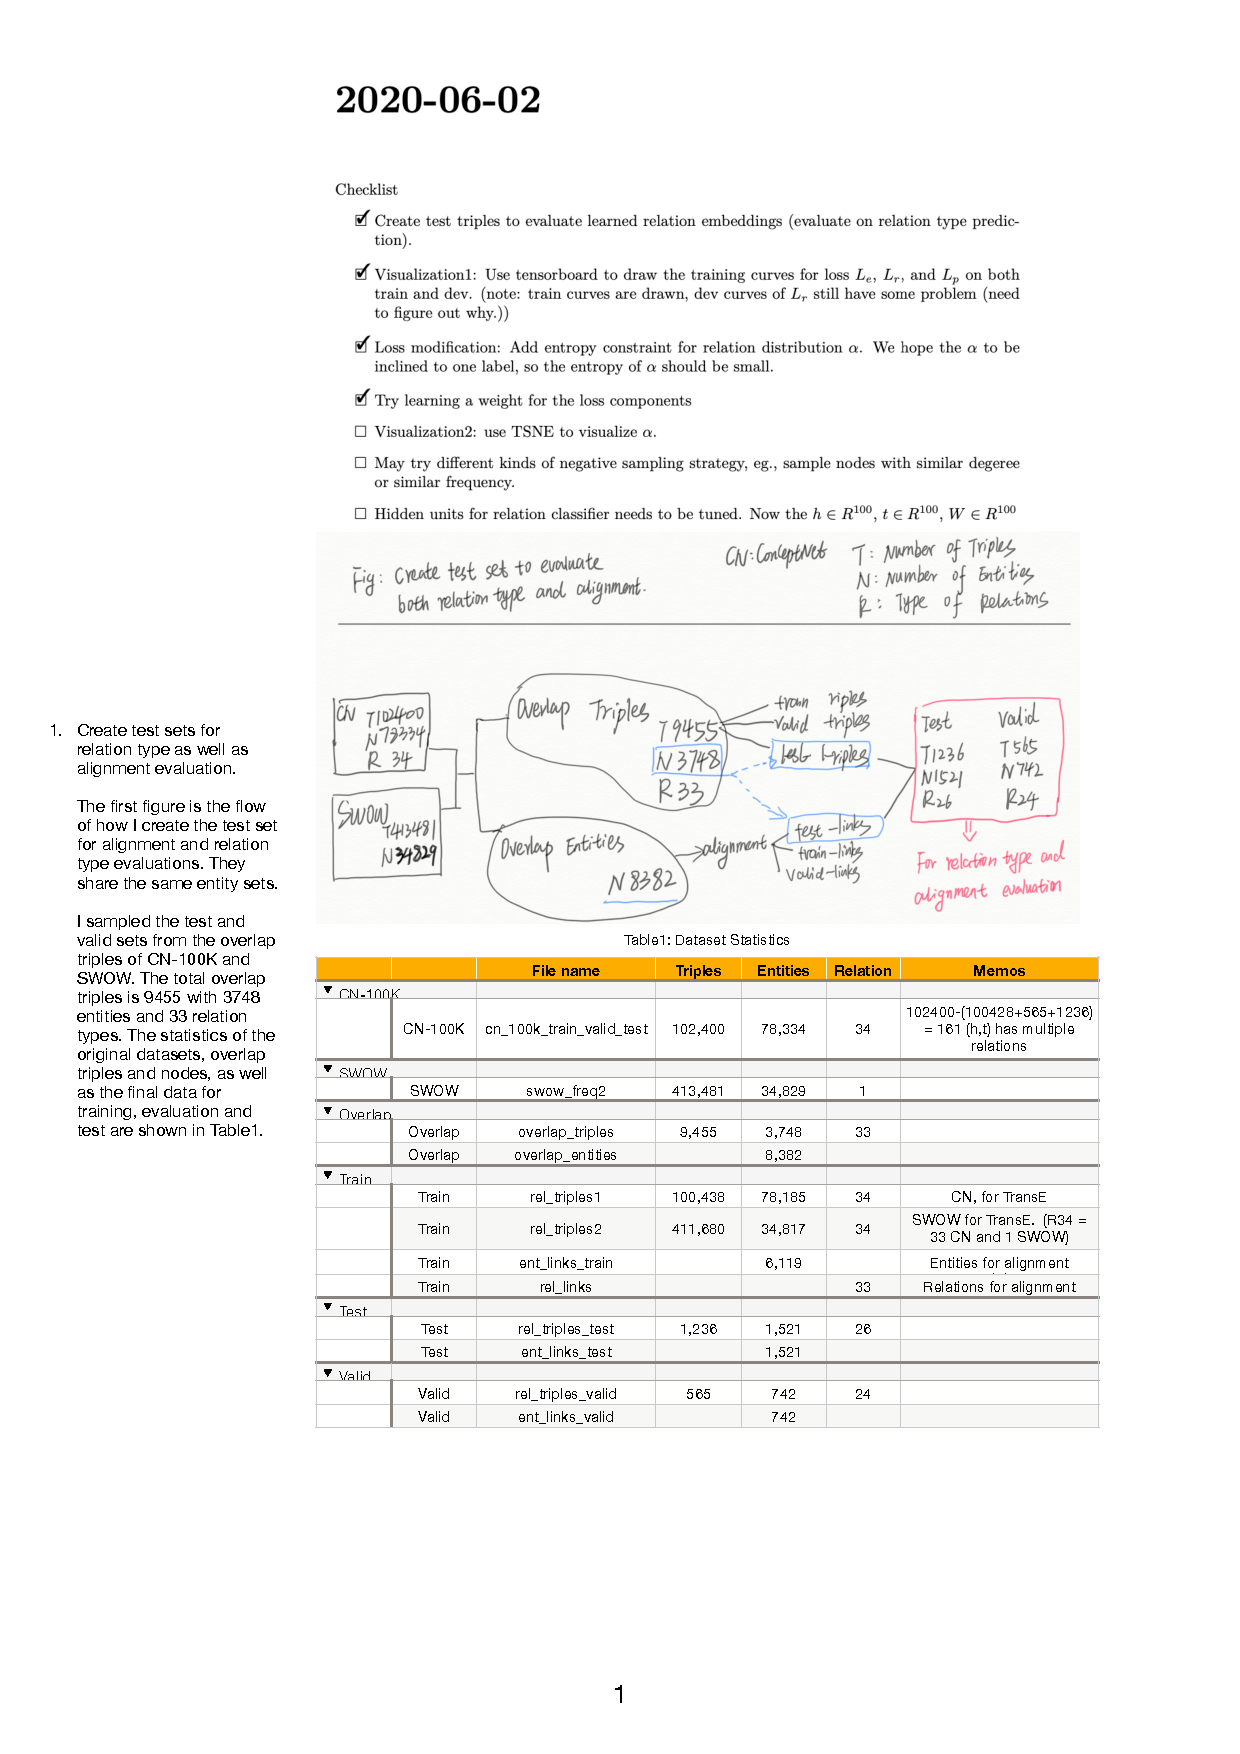
\includepdf[]{images/2020-06-02.pdf}
\clearpage
\section{Meeting Notes}
\textbf{To do list}
\begin{enumerate}
    \item For valid sets:
        \begin{enumerate}
            \item Figure out why hits and mrr on valid set is much lower than test set. 
            \item Visualize training curves on valid set. 
        \end{enumerate}
    \item Add evaluation on link prediction ($p(t|h,r)$) and triple classification (p(h,r,t) whether a triple exists).
    \item Add one more baseline: add the relation calssifier on TransE model and evaluate it. 
    \item Analysis on $\beta_1$ and $\beta_2$: 
    \begin{enumerate}
        \item Zoom in current $\beta_1$ (0-0.1) and $\beta_2$ (0.1-0.2) to see how they influce the MRR and the  REL\_ACC 
        \item Scale up the $\beta_1$ and $\beta_2$ to balance the scale range between $L_r$ and $L_p$ with $L_e$. (Because $L_e \approx 5*L_r$ and $L_e \approx 10*L_p$.) 
        \item Draw the correlation between $\beta_1$ and $\beta_2$ with the evaluation matrics. Observe how $\beta_1$ and $\beta_2$ influence the MRR or REL\_ACC.
    \end{enumerate}
    \item Print the confusion matrix for relation types to observe how model performs on each type.
    \item Apply dropout to model to tackle the overfitting problem of relaiton type accuracy.  
\end{enumerate} 